\chapter{Analisi}
\label{cap:analisi}

\intro{In questo capitolo si approfondisce in dettaglio il funzionamento del framework OpenVLC, le minacce alla sicurezza a cui è soggetto e le possibili contromisure. Si descrive inoltre la configurazione dell'ambiente nell'ambito del progetto e le problematiche riscontrate.}\\

% ================================================================= %
\section{Analisi della piattaforma OpenVLC}

\paragraph{Introduzione.}
OpenVLC\footcite{site:openvlc} è una piattaforma open source per la comunicazione ottica wireless, sviluppata dal Pervasive Wireless Systems group del Dr. Giustiniano all'IMDEA Networks Institute (Madrid, Spagna).
OpenVLC è progettata per consentire agli sviluppatori di sperimentare con la \gls{vlc}, per essere flessibile e low-cost, permettendo, nell'ultima versione, la trasmissione di dati ad una velocità di 400 kb/s e ad una distanza di quasi 20 metri.

\paragraph{Motivazioni.}
Si è scelto di utlizzare OpenVLC proprio a causa della sua accessibilità e popolarità. Infatti, nonostante sia un progetto di piccole dimensioni, possiede delle caratteristiche, come ad esempio l'essere open source e l'avere una community di discrete dimensioni, che lo rendono la soluzione ideale, e probabilemente l'unica, per la ricerca in ambito \gls{vlc}.\\
È infatti importante evidenziare, che durante lo svolgimento del progetto, a causa di problematiche riscontrate nella configurazione delle due schede BeagleBone, si è valutata l'idea di trovare un'alternativa ad OpenVLC. Si è considerato, ad esempio, l'utilizzo di un software diverso o addirittura di un qualche programma che permettesse di simulare una comunicazione tramite luce visibile. Tuttavia a seguito di varie ricerche, si è concluso che OpenVLC fosse l'unica soluzione open source attualmente in circolazione.

\paragraph{Hardware.}
OpenVLC si appoggia su schede BeagleBone\footcite{site:beaglebone}Black, una piattaforma hardware open source low-cost per sviluppatori, dotata di un processore ARM Cortex-A8 e di una serie di interfacce di comunicazione, tra cui USB, Ethernet e GPIO. BeagleBone è particolarmente adatta per applicazioni embedded e IoT, grazie alla sua flessibilità e alle sue capacità di elaborazione.\\
La seconda componente hardware fondamentale per il funzionamento di OpenVLC è l'\textit{OpenVLC1.3 cape}, una scheda di espansione progettata per la BeagleBone Black. Questo cape integra i circuiti necessari per la trasmissione e la ricezione di segnali luminosi, includendo un LED per l'emissione e un fotodiodo per la ricezione. Inoltre, il cape dispone di circuiti di amplificazione e filtraggio per garantire una comunicazione affidabile e ridurre il rumore di fondo. L'interfaccia tra la BeagleBone e il cape avviene tramite i pin GPIO, permettendo una gestione diretta dei segnali ottici tramite software.

\paragraph{Driver e Sistema Operativo.}
% come funziona l'ambiente di OpenVLC (descrizione ad alto livello del sistema)
Il codice sorgente di OpenVLC è formato da due componenti: il software necessario a gestire i livelli \gls{phy} e \gls{mac} e ad interfacciarli con i livelli superiori del modello \gls{osi}; il firmware necessario a controllare i \gls{pru} delle schede BeagleBone.\\
Nella versione 1.3 è stata introdotta la possibilità di utilizzare anche un LED infrarossi per trasmettere dati, il quale può affiancare il classico LED oppure essere usato singolarmente.
Di conseguenza, nel caso del trasmettitore, il framework può essere selezionato tra varie possibilità a seconda del livello di dimming desiderato. Ovvero in funzione di quanto si desidera usare il LED VL piuttosto che il LED IR.
Di seguito le possibili opzioni fornite in OpenVLC:
\begin{itemize}
    \item 0\% Dimming (solo luce visibile)
    \item 25\% Dimming
    \item 50\% Dimming
    \item 75\% Dimming
    \item 100\% Dimming (solo infrarossi)
\end{itemize}
Nell'ambito del progetto qui presentato, trattandosi di \gls{vlc}, si è deciso di usare la prima opzione, ovvero solo luce visibile.

In figura \ref{fig:beaglebone_cape} si possono osservare una scheda BeagleBone Black (a sinistra) ed un \textit{OpenVLC1.3 cape}. Sul cape \textit{IR LED} indica il LED infrarossi, \textit{VL LED} indica il LED visible light e \textit{PD} indica il fotodiodo ricevitore.
\begin{figure}[H] 
    \centering 
    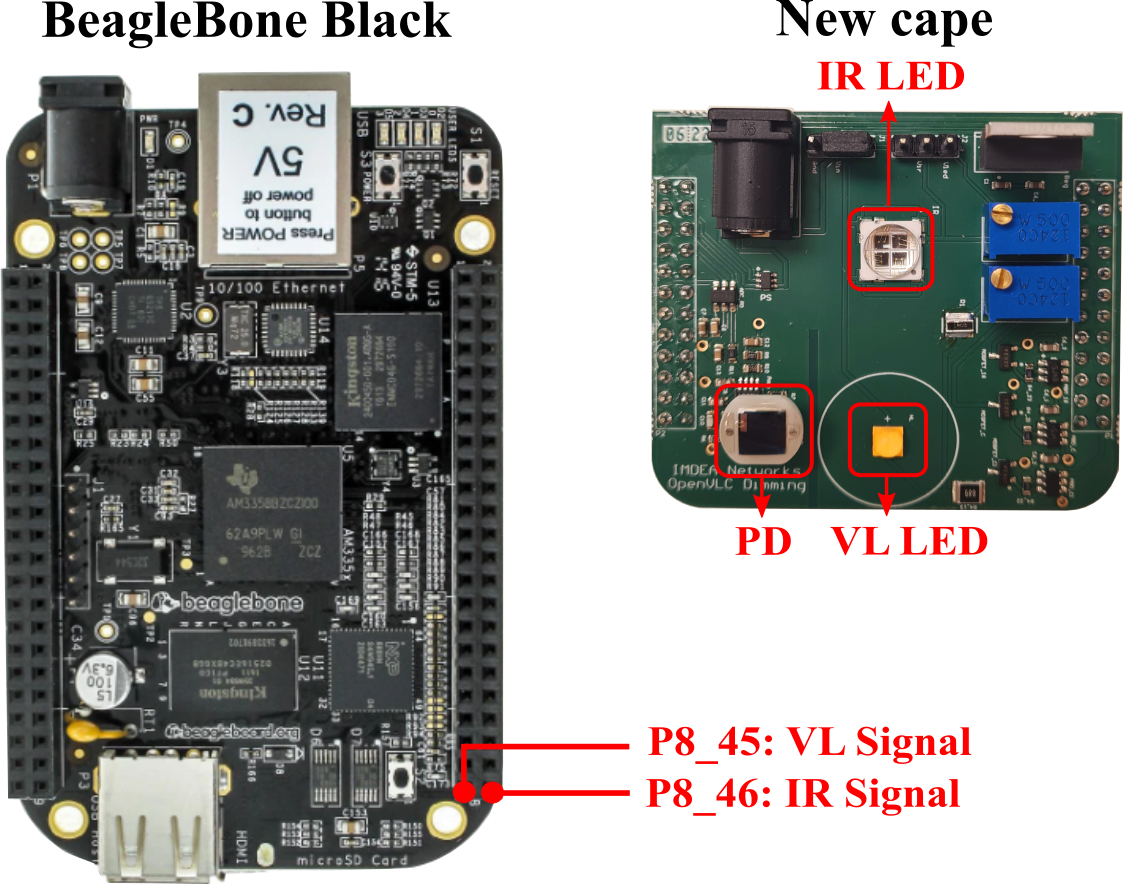
\includegraphics[width=0.9\columnwidth]{openvlc/Cape_for_TX_in_VL_IR_bands}
    \caption{Test iperf riportato nella documentazione di OpenVLC}
    \label{fig:beaglebone_cape}
\end{figure}

Durante la configurazione, sulle schede BeagleBone, viene installato il sistema operativo \textit{Debian 8 "jessie"}. Il driver di OpenVLC è di fatto un modulo del kernel \textit{Linux} che agisce da ponte tra lo stack di rete del sistema operativo e l'hardware BeagleBone.

\paragraph{Reti e Sicurezza.}
Una volta configurate correttamente due schede, la prima come trasmettitore e la seconda come ricevitore, è quindi possibile usarle come una \textit{common network interface}. Ovvero il sistema operativo, in questo caso Debian 8, può usare OpenVLC allo stesso modo in cui userebbe una normale interfaccia di rete, come ad esempio inviare/ricevere pacchetti IP e comunicare con altri dispositivi su una rete locale.\\
Come già anticipato, ognuna delle due schede ha uno ed un solo ruolo, non è infatti possibile attualmente trasmettere e ricevere dalla stessa scheda contemporaneamente. Questo tipo di canale di comunicazione viene denominato \textit{simplex} (unidirezionale), in contrapposizione ad esempio ad un canale \textit{duplex} in cui un device può cambiare ruolo dinamicamente o ad un canale \textit{full-duplex} in cui un device può trasmettere e ricevere simultaneamente.\\
In OpenVLC, per cambiare il ruolo di un device, bisogna di fatto ricompilare il driver.

OpenVLC, essendo un progetto di piccole dimensioni ed avendo come obbiettivo quello di sperimentare con la \gls{vlc}, piuttosto che usarla per comunicazioni realistiche, non implementa delle vere e proprie reti o un infrastruttura hardware/software che permetta di implementare delle reti di calcolatori.

Per quanto riguarda invece la sicurezza, il driver di OpenVLC, gestendo i livelli \gls{phy} e \gls{mac}, non implementa alcun meccanismo di sicurezza. Lascia invece che questa sia gestita dai livelli superiori. Tuttavia definire protocolli di sicurezza a livello fisico è decisamente utile, in particolar modo se si considera che la \gls{vlc} viene utilizzata in contesti in cui la sicurezza delle reti di comunicazione è critica, come ad esempio ospedali e convogli di veicoli.

In figura \ref{fig:design_openvlc} si riporta uno schema riassuntivo dell'architettura di OpenVLC in cui si può osservare quanto descritto precedentemente.
\begin{figure}[H] 
    \centering 
    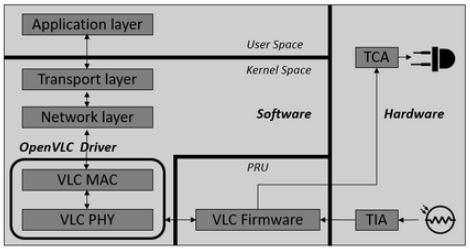
\includegraphics[width=0.9\columnwidth]{openvlc/design_openvlc}
    \caption{Architettura di OpenVLC}
    \label{fig:design_openvlc}
\end{figure}

\paragraph{PHY Frame e Modulazioni.}

















% struttura PHY frame (e OSI in generale in standard?)
% spiega le varie parti del frame come devono essere modulate secondo lo standard e secondo openvlc


\subsection{Configurazione e problematiche riscontrate}
% descrivere la versione di OpenVLC usata e come è stato configurato il sistema
% descrivi anche le problematiche riscontrate durante la configurazione e come le hai risolte
% di che per com'è scritto il codice ci sono gravi problemi di sincronizzazione dato che la ricezione del preambolo è commentata
% installazione os e script fatti per automatizzare la configurazione


% ================================================================= %
\section{Vulnerabilità}
% possibili attacchi e Vulnerabilità
% cosa assumi sull'attaccante: posizione buona per intercettare il fascio, rubare i pacchet-
% ti, rubare le password, modificare pacchetti, distruggere pacchetti a caso o mandare
% pacchetti a caso

% ================================================================= %
\section{Soluzione proposta}
% vedi phyauth fine cap 1
% spiega come funziona l'autenticazione a livello fisico.
% vantaggi della soluzione proposta